Given a snowflake in arbirary position with $n$ unit segments per arm, the arms of the snowflake has a maximal length of $n$, end to end, if in canonical position; otherwise, the arm will have an end to end length less than $n$ (See Figure \ref{fig:LineSegmentDelta.pdf}).  
The arm of a snowflake in arbitrary position corresponds to a compression and shift of vertices.  


\begin{minipage}{\linewidth}
\begin{center}
\includegraphics[width=.95\columnwidth]{graphics/LineSegmentDelta.pdf}
\captionof{figure}{The polyline at the bottom represents a snowflake arm in canonical position.  The polyline above represents a snowflake arm in non-canonical position.}\label{fig:LineSegmentDelta.pdf}
\end{center}
\end{minipage}

We will show for any $\epsilon >0$ and arbitrary position of vertices, the placement of vertices is close to canonical position.  
In order to show this, we show the components of a perturbed snowflake in arbitrary position  are close to canonical position.  
The argument comprises of three parts: (1) Showing that the pertubation of $S_1$ is small, (2) show that the displacement along the arms for all $S_i$ for $i \geq 1$ is small, and (3) show that the displacement along the petioles is small.  

\paragraph{Displacement on $S_1$ is small.}
Suppose we are given an ordered weighted tree $T_\epsilon$ such that the corresponding disk arrangement is a perturbed $S_1$.  
In a perfect snowflake of $S_1$ the six disks around the central disk kiss each other.  
The angle formed from the center of the central disk to the centers of any two adjacent disks is $\frac{\pi}{3}$.  
The side lengths of the equalateral triangle formed by the centers of three adjacent disks, one of which is the central disk, is $2r$.  
For a perturbed $S_1$ the the central disk is weighted $r+ \epsilon$.  
This can yield a change of angular displacement from $\frac{\pi}{3}$ to $\frac{\pi}{3} + 2\chi$.  
To find the bounds of how large or small $\chi$ can be, we show the trigonometric relation of the half angle of the triangle corresponding to three adjacent disks (See Figure \ref{fig:part1ch4.pdf}):
\begin{eqnarray*}
\sin \lr{\frac{\pi}{6} - \chi} &=& \frac{1}{2r+\epsilon}\\
\sin \frac{\pi}{6} \cos \chi &=& \frac{1}{2r+\epsilon} + \cos \frac{\pi}{6} \sin \chi\\
&\iff&\\
\frac{1}{2} &\geq& \frac{1}{2} \cos \chi \\
&=& \frac{1}{2r+\epsilon} + \frac{\sqrt{3}}{2} \sin \chi\\
&\geq& \frac{1}{2r+\epsilon} + \frac{\sqrt{3}}{2} \lr{ \chi - \frac{\chi^3}{6}}\\
&\iff&\\
\frac{1}{2}-\frac{1}{2r+\epsilon} &\geq& \frac{\sqrt{3}}{2} \lr{ \chi - \frac{\chi^3}{6}} \qquad \text{if }\chi < 1\\
\frac{2r + \epsilon - 2}{2 ( 2 + \epsilon)} &\geq&  \frac{5\sqrt{3}}{12} \chi\\
&&\text{for $r=1$}\\
\frac{3 \epsilon}{5\sqrt{3}}=\frac{12}{5\sqrt{3}} \frac{\epsilon}{4} &\geq& \chi
\end{eqnarray*}

\begin{minipage}{\linewidth}
\begin{center}
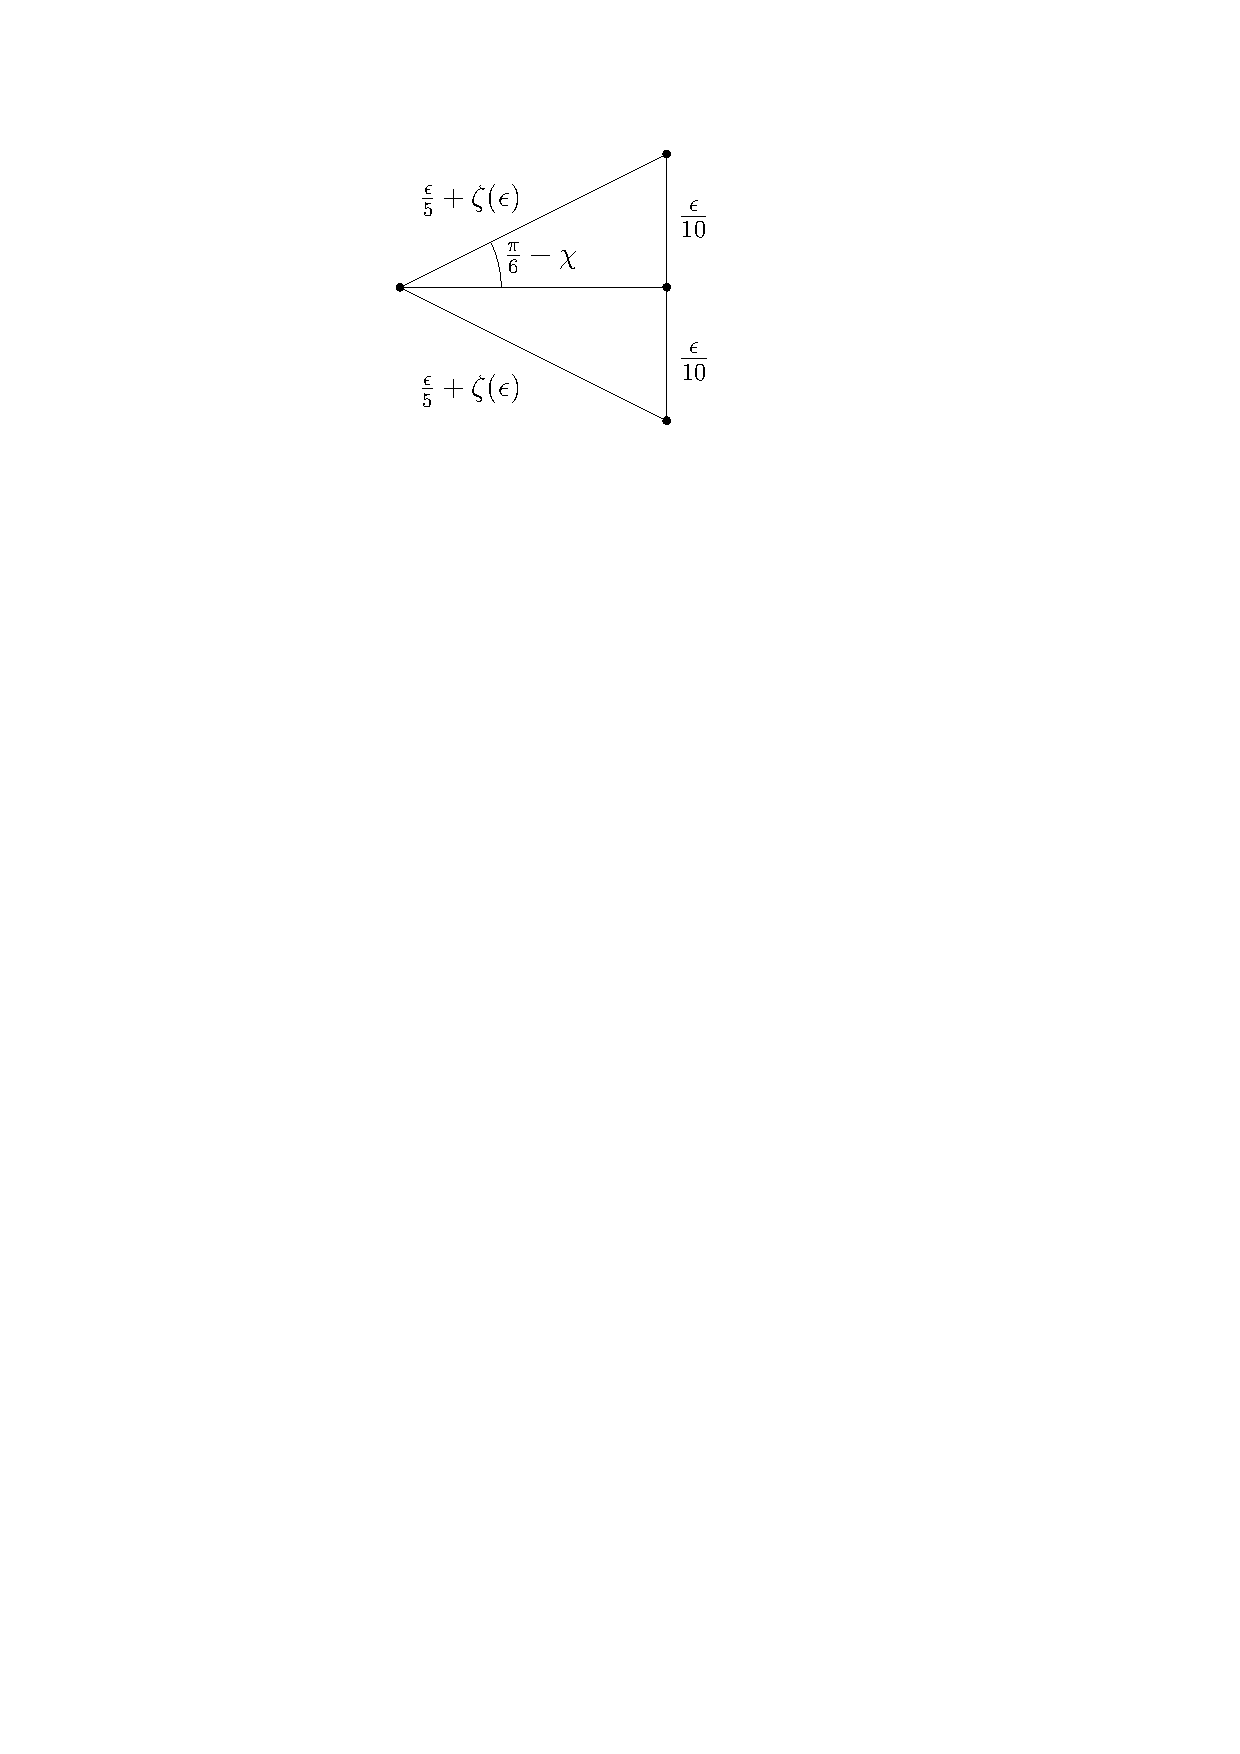
\includegraphics[width=.20\columnwidth]{graphics/part1ch4.pdf}
\captionof{figure}{This figure depicts a triangle corresponding to the center of the central disk and two adjacent disks.}\label{fig:part1ch4.pdf}
\end{center}
\end{minipage}

For any $\epsilon > 0$, the bounds for angular displacement formed at the center of the central disk and two adjacent disks is:
$$ \frac{\pi}{3} - \frac{6 \epsilon}{5\sqrt{3}} \leq \frac{\pi}{3} - 2 \chi = \lambda_\text{min} \leq \lambda \leq \lambda_\text{max} = \frac{\pi}{3} + 2 \chi \leq \frac{\pi}{3} + \frac{6 \epsilon}{5\sqrt{3}}$$
\paragraph{Displacement on the arms is small.}
To show that the angluar displacement along the arm is small, we extend the angular argument on the perturbed $S_1$ and by induction, show that it is small for all $i$.  

\begin{minipage}{\linewidth}
\begin{center}
\includegraphics[width=.5\columnwidth]{graphics/Vertebrae.pdf}
\captionof{figure}{An arm depicted at the $\ith$ and $(i+1)^\text{st}$ vertex.}\label{fig:Vertebrae.pdf}
\end{center}
\end{minipage}

Denote the angles on the concave side of the $\ith$ vertex as $\alpha_i$ and $\beta_i$ and the convex side of the $(i+1)^\text{st}$ vertex as $\gamma_i$ and $\delta_i$ respectively (see Figure \ref{fig:Vertebrae.pdf} for reference). 

For any vertex, the sum of angles about the vertex is $2 \pi$, e.g.:
$$\gamma_i + \delta_i + \alpha_{i+1} + \beta_{i+1} = 2 \pi$$ 

Suppose we numbered the the disks about the central disk 1 through 6.  
Without loss of generality, the angles $\alpha_0$ and $\beta_0$ correspond to the angles formed between the central angle, disks $i$ and $i+1$ and disks $i+1$ and $i+2$ respectively, for $i = 1,2,3$.  
The bounds for $\alpha_0$ and $\beta_0$ are the same as $\lambda$ in the earlier argument, i.e.:
$$
\begin{array}{rcccl}
\frac{\pi}{3} - \frac{6 \epsilon}{5\sqrt{3}} &\leq& \alpha_0 &\leq& \frac{\pi}{3} + \frac{6 \epsilon}{5\sqrt{3}}\\
\frac{\pi}{3} - \frac{6 \epsilon}{5\sqrt{3}} &\leq& \beta_0 &\leq& \frac{\pi}{3} + \frac{6 \epsilon}{5\sqrt{3}}\\
\end{array}
$$

We know that $\alpha_0 + \beta_0 \leq \frac{2\pi}{3} + \frac{12\epsilon}{5\sqrt{3}}.$
We also know that in canonical position:
$$ 
\begin{array}{rcl}
\pi &=& \alpha_0 + \gamma_0 \\
\pi &=& \beta_0 + \delta_0
\end{array}
$$
Together, we have the following result:
\begin{eqnarray*}
2\pi &=& \alpha_0 + \gamma_0 + \beta_0 + \delta_0\\
2\pi &=& \alpha_0 + \gamma_0 + \lr{2\pi - \alpha_1 - \beta_1}\\
\alpha_1 + \beta_1&=&\alpha_0 + \gamma_0 \\
&\leq& \frac{2\pi}{3} + \frac{12\epsilon}{5\sqrt{3}}\\
\end{eqnarray*}
And so the error bounds on $\lambda$ hold in general for $\alpha_i$ and $\beta_i$ for all $i$.  
\paragraph{Displacement on the petioles is small.}
Note that the petioles have the same geometric structure as the arms; the exception is the number of leafs on each side of the petioles. 
Since we've shown that the geometric shape in arbirary position is already close to canonical position for any $\epsilon>0$, the same argument applies here for the petioles.

We have shown the displacements of all components of the perturbed snowflake are small for any $\epsilon > 0$.  
This shows that the structure has stability in preserving any information encoded with it.










